\chapter{Theoretical background}

\section{Structure-from-Motion}
\label{sec:sfm}

Structure-from-Motion (SfM) is a foundational technique in computer vision that recovers three-dimensional scene structure and camera motion from multiple two-dimensional images. Given a set of images of a static scene captured from different viewpoints, SfM jointly estimates camera intrinsics, camera poses, and a sparse 3D point cloud by exploiting multi-view geometric constraints.

\subsection{Pinhole Camera Model}

The pinhole camera model provides a mathematical abstraction of image formation. A 3D point in world coordinates is represented in homogeneous form as
\begin{equation}
\mathbf{X} = (X, Y, Z, 1)^\top.
\end{equation}
The projection of $\mathbf{X}$ onto the image plane is given by
\begin{equation}
\mathbf{x} \sim \mathbf{P} \mathbf{X},
\end{equation}
where $\mathbf{x} = (u, v, 1)^\top$ denotes a homogeneous image point, and $\mathbf{P}$ is the $3 \times 4$ camera projection matrix.

The projection matrix can be decomposed as
\begin{equation}
\mathbf{P} = \mathbf{K} [\mathbf{R} \mid \mathbf{t}],
\end{equation}
where $\mathbf{R} \in SO(3)$ and $\mathbf{t} \in \mathbb{R}^3$ represent the camera rotation and translation from world to camera coordinates. The intrinsic calibration matrix $\mathbf{K}$ is defined as
\begin{equation}
\mathbf{K} =
\begin{bmatrix}
f_x & s & c_x \\
0 & f_y & c_y \\
0 & 0 & 1
\end{bmatrix},
\end{equation}
with focal lengths $f_x, f_y$, skew parameter $s$, and principal point $(c_x, c_y)$. In most modern datasets, the skew is assumed to be zero.

In camera coordinates, the perspective projection is expressed as
\begin{equation}
\begin{bmatrix}
x \\ y \\ z
\end{bmatrix}
=
\mathbf{R}
\begin{bmatrix}
X \\ Y \\ Z
\end{bmatrix}
+
\mathbf{t},
\end{equation}
followed by normalization:
\begin{equation}
u = \frac{x}{z}, \quad v = \frac{y}{z}.
\end{equation}
This non-linear division by depth $z$ is the fundamental source of projective ambiguity in monocular reconstruction.

\subsection{Two-View Geometry and Epipolar Constraint}

Consider two pinhole cameras observing the same 3D point $\mathbf{X}$, producing image projections $\mathbf{x}_1$ and $\mathbf{x}_2$. The relative camera motion induces a geometric constraint known as epipolar geometry.

Let $\mathbf{C}_1$ and $\mathbf{C}_2$ denote the camera centers. The baseline connecting the two centers, together with $\mathbf{X}$, defines the epipolar plane. The intersection of this plane with each image plane yields an epipolar line. Consequently, the projection of $\mathbf{X}$ in one image must lie on the epipolar line corresponding to its projection in the other image.

This relationship is algebraically encoded by the fundamental matrix $\mathbf{F}$:
\begin{equation}
\mathbf{x}_2^\top \mathbf{F} \mathbf{x}_1 = 0.
\end{equation}
For a fixed point $\mathbf{x}_1$, the corresponding epipolar line in the second image is given by
\begin{equation}
\mathbf{l}_2 = \mathbf{F} \mathbf{x}_1.
\end{equation}

The epipoles $\mathbf{e}_1$ and $\mathbf{e}_2$ are defined as the projections of the opposite camera centers onto each image plane and satisfy
\begin{equation}
\mathbf{F} \mathbf{e}_1 = \mathbf{0}, \quad \mathbf{e}_2^\top \mathbf{F} = \mathbf{0}.
\end{equation}

\subsection{Essential Matrix and Relative Pose Recovery}

If the intrinsic calibration matrices $\mathbf{K}_1$ and $\mathbf{K}_2$ are known, the epipolar constraint can be expressed in normalized image coordinates using the essential matrix $\mathbf{E}$:
\begin{equation}
\mathbf{E} = \mathbf{K}_2^\top \mathbf{F} \mathbf{K}_1.
\end{equation}
The essential matrix has rank 2 and can be decomposed as
\begin{equation}
\mathbf{E} = [\mathbf{t}]_\times \mathbf{R},
\end{equation}
where $[\mathbf{t}]_\times$ is the skew-symmetric matrix corresponding to the translation vector. Decomposition of $\mathbf{E}$ yields up to four possible solutions for $(\mathbf{R}, \mathbf{t})$, which are disambiguated by enforcing positive depth constraints during triangulation.

\subsection{Triangulation and Reprojection Error}

Given camera projection matrices $\mathbf{P}_i$ and corresponding observations $\mathbf{x}_i$, the 3D point $\mathbf{X}$ is estimated by triangulation. In practice, triangulation is performed by minimizing the reprojection error:
\begin{equation}
\min_{\mathbf{X}} \sum_i \left\| \mathbf{x}_i - \pi(\mathbf{P}_i \mathbf{X}) \right\|^2,
\end{equation}
where $\pi(\cdot)$ denotes homogeneous normalization. Reprojection error serves as the primary geometric objective throughout the SfM pipeline.

\subsection{Global Optimization via Bundle Adjustment}

To achieve a consistent reconstruction across all views, SfM employs bundle adjustment, a joint non-linear optimization over camera parameters and 3D points:
\begin{equation}
\min_{\{\mathbf{R}_i, \mathbf{t}_i, \mathbf{X}_j\}} 
\sum_{i,j} \left\| \pi(\mathbf{K}_i (\mathbf{R}_i \mathbf{X}_j + \mathbf{t}_i)) - \mathbf{x}_{ij} \right\|^2.
\end{equation}
This optimization refines camera poses, intrinsics, and 3D structure simultaneously, significantly improving geometric accuracy.

\subsection{COLMAP as a Practical SfM System}

COLMAP is a widely used SfM and Multi-View Stereo pipeline that implements an incremental SfM strategy with robust feature matching, epipolar verification, and large-scale bundle adjustment. Given an unordered set of images, COLMAP estimates camera intrinsics and extrinsics, reconstructs a sparse point cloud, and outputs calibrated camera poses.

In neural and Gaussian-based scene representations, including 3D Gaussian Splatting and its geometry-aware extensions, COLMAP serves as the standard tool for camera pose initialization. While COLMAP provides highly accurate pose estimates, the resulting point cloud remains sparse and does not explicitly encode surface continuity or structural priors such as planar geometry. These limitations motivate the integration of additional geometric constraints in downstream representations, including planar primitives, depth supervision, and multi-view stereo cues, as explored in PlanarGS and related methods.


\section{3D Gaussian Splatting}

\subsection{Overview}

3D Gaussian Splatting (3DGS) is a point-based neural rendering method that represents a scene as a set of anisotropic 3D Gaussian primitives. Instead of using implicit neural fields, the scene geometry and appearance are explicitly modeled using a collection of volumetric Gaussians that are optimized directly through differentiable rendering.

The key idea is to approximate the scene with a set of Gaussian functions that are projected onto the image plane and composited using alpha blending.

\begin{figure}[t]
    \centering
    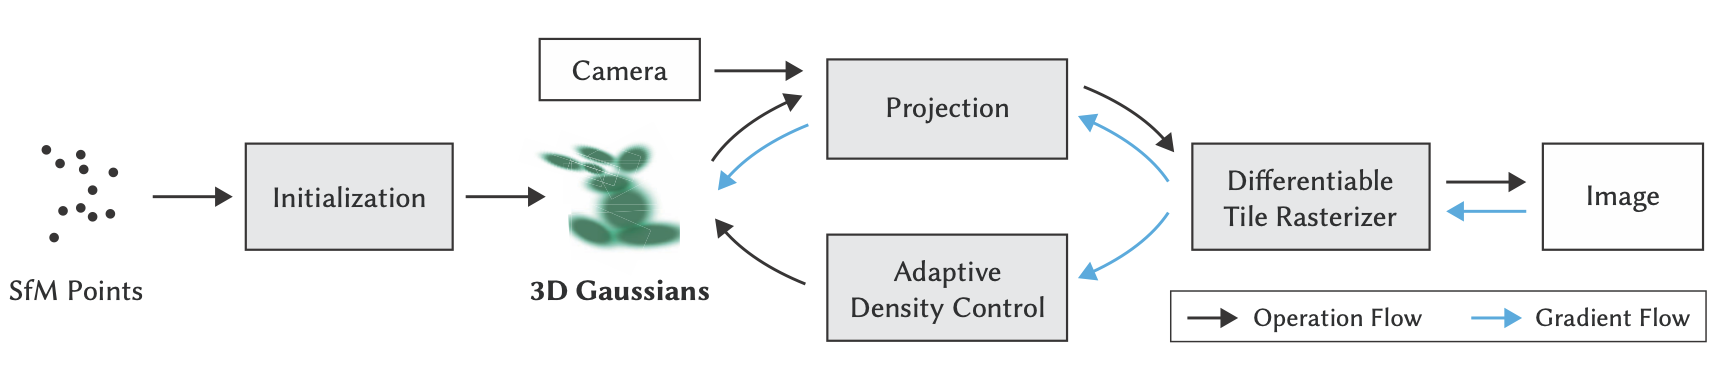
\includegraphics[width=\textwidth]{3DGSWorkflow.png}
    \caption{Overview of the 3D Gaussian Splatting pipeline. The workflow illustrates scene initialization, Gaussian optimization, and real-time rendering via splatting and alpha compositing. Image reproduced from the original 3D Gaussian Splatting paper by Kerbl et al.~\cite{kerbl20233dgs}.}
    \label{fig:3dgs_workflow}
\end{figure}

\subsection{Gaussian Representation}

A scene is represented as a set of $N$ Gaussians:

\[
\mathcal{G} = \{ G_i \}_{i=1}^{N}
\]

Each Gaussian $G_i$ is defined by:

\[
G_i = (\boldsymbol{\mu}_i, \boldsymbol{\Sigma}_i, \alpha_i, \mathbf{c}_i)
\]

where:
\begin{itemize}
    \item $\boldsymbol{\mu}_i \in \mathbb{R}^3$ is the 3D mean (center),
    \item $\boldsymbol{\Sigma}_i \in \mathbb{R}^{3 \times 3}$ is the covariance matrix,
    \item $\alpha_i \in [0,1]$ is the opacity,
    \item $\mathbf{c}_i$ are color coefficients (typically spherical harmonics).
\end{itemize}

The spatial density of a Gaussian is defined as:

\[
\mathcal{N}(\mathbf{x}; \boldsymbol{\mu}_i, \boldsymbol{\Sigma}_i)
=
\exp \left(
-\frac{1}{2}
(\mathbf{x} - \boldsymbol{\mu}_i)^\top
\boldsymbol{\Sigma}_i^{-1}
(\mathbf{x} - \boldsymbol{\mu}_i)
\right).
\]

\subsection{Projection and Rendering}

For a camera with projection function $\pi(\cdot)$, each 3D Gaussian is projected into image space. Due to perspective projection, the Gaussian remains Gaussian in 2D with projected mean and covariance:

\[
\mathbf{u}_i = \pi(\boldsymbol{\mu}_i)
\]

The rendered color at pixel $\mathbf{u}$ is computed using alpha compositing:

\[
C(\mathbf{u}) = \sum_{i} T_i(\mathbf{u}) \alpha_i(\mathbf{u}) \mathbf{c}_i,
\]

where the accumulated transmittance is:

\[
T_i(\mathbf{u}) = \prod_{j < i} \left(1 - \alpha_j(\mathbf{u}) \right).
\]

The Gaussians are sorted in front-to-back order according to depth.

\subsection{Optimization Objective}

The parameters of all Gaussians are optimized by minimizing a photometric reconstruction loss between rendered and ground-truth images:

\[
\mathcal{L}_{rgb}
=
\sum_{\mathbf{u}}
\| C(\mathbf{u}) - I_{gt}(\mathbf{u}) \|_1.
\]

Additional regularization terms such as depth consistency or normal consistency can be incorporated:

\[
\mathcal{L}_{total}
=
\mathcal{L}_{rgb}
+
\lambda_{depth} \mathcal{L}_{depth}
+
\lambda_{normal} \mathcal{L}_{normal}.
\]

\subsection{Adaptive Densification}

To increase representational capacity in complex regions, 3DGS performs adaptive densification. A Gaussian is split when the magnitude of the gradient with respect to its center exceeds a threshold:

\[
\| \nabla_{\boldsymbol{\mu}_i} \mathcal{L}_{total} \| > \gamma.
\]

This mechanism increases the number of Gaussians in high-frequency regions such as edges or textured areas while keeping flat regions compact.

\subsection{Advantages}

Compared to neural radiance fields, 3D Gaussian Splatting:
\begin{itemize}
    \item Enables real-time rendering,
    \item Uses explicit geometric primitives,
    \item Avoids expensive volumetric ray marching,
    \item Allows adaptive refinement through splitting and pruning.
\end{itemize}


\section{Geometry Priors in Gaussian Splatting}
\label{sec:geometry_priors}

While 3D Gaussian Splatting provides an explicit and efficient scene representation, its optimization is primarily driven by photometric supervision. Purely image-based supervision can lead to geometric artifacts such as floaters, inconsistent surface orientation, and poor reconstruction in textureless regions. To address these limitations, additional geometric priors can be incorporated into the training process. These priors introduce structural constraints that improve geometric consistency and stability.

\subsection{Depth Priors}

Depth priors provide direct supervision on scene geometry. Depth information can be obtained from multi-view stereo (MVS) methods, LiDAR sensors, or monocular depth estimation networks.

Let $D_{render}(\mathbf{u})$ denote the depth rendered from the Gaussian representation and $D_{prior}(\mathbf{u})$ the externally estimated depth map. A common supervision term is defined as:

\begin{equation}
\mathcal{L}_{depth}
=
\sum_{\mathbf{u} \in \Omega}
\left|
D_{render}(\mathbf{u}) - D_{prior}(\mathbf{u})
\right|,
\end{equation}

where $\Omega$ represents the set of pixels with reliable depth values.

Depth supervision improves geometric accuracy, reduces floating artifacts, and stabilizes optimization in low-texture regions. However, noisy depth estimates must often be filtered using geometric verification or confidence masks.

\subsection{Normal Priors}

Surface normal priors enforce orientation consistency of reconstructed surfaces. Normals can be derived from depth maps or predicted using monocular normal estimation networks.

Let $\mathbf{n}_{render}(\mathbf{u})$ denote the normal estimated from the rendered Gaussian surface and $\mathbf{n}_{prior}(\mathbf{u})$ the reference normal. A cosine similarity loss is commonly used:

\begin{equation}
\mathcal{L}_{normal}
=
\sum_{\mathbf{u}}
\left(
1 - 
\mathbf{n}_{render}(\mathbf{u})^\top
\mathbf{n}_{prior}(\mathbf{u})
\right).
\end{equation}

Normal constraints improve local surface smoothness and reduce geometric noise, particularly in planar or weakly textured regions.

\subsection{Mesh-Based Priors}

When an approximate surface mesh is available (e.g., reconstructed from MVS), it can serve as a geometric regularizer. Gaussians can be constrained to remain close to the mesh surface.

Let $\mathcal{M}$ denote a reference mesh and $\text{dist}(\boldsymbol{\mu}_i, \mathcal{M})$ the shortest distance from a Gaussian center to the mesh surface. A regularization term can be defined as:

\begin{equation}
\mathcal{L}_{mesh}
=
\sum_{i}
\text{dist}(\boldsymbol{\mu}_i, \mathcal{M})^2.
\end{equation}

This prior enforces surface adherence and improves global geometric consistency. It is particularly useful in structured environments where reliable coarse geometry can be extracted.

\subsection{Edge and Line Priors}

Image edges and line segments encode strong structural cues about scene geometry. Line detection methods can extract 2D line segments, which can be matched across views to recover 3D line constraints.

Let $\mathbf{l}_{render}$ denote projected Gaussian-induced edges and $\mathbf{l}_{obs}$ detected image lines. An alignment loss may penalize angular deviation or distance between projected and observed lines:

\begin{equation}
\mathcal{L}_{edge}
=
\sum_{k}
\left\|
\mathbf{l}_{render}^{(k)} -
\mathbf{l}_{obs}^{(k)}
\right\|.
\end{equation}

Edge-based priors improve reconstruction of sharp structures such as building edges, corners, and object boundaries, which are often smoothed by purely photometric optimization.

Incorporating geometric priors transforms Gaussian Splatting from a purely photometric renderer into a geometry-aware representation capable of producing structurally consistent reconstructions.



\section{Quality Metrics}
\label{sec:quality_metrics}

To quantitatively evaluate the visual quality of the reconstructed images, we employ several commonly used image quality metrics: Peak Signal-to-Noise Ratio (PSNR), Structural Similarity Index Measure (SSIM), and Learned Perceptual Image Patch Similarity (LPIPS). These metrics capture complementary aspects of reconstruction quality, ranging from pixel-wise accuracy to perceptual similarity, and are widely adopted in neural rendering and view synthesis literature~\cite{mildenhall2020nerf,kerbl20233dgs}.

\subsection{Peak Signal-to-Noise Ratio (PSNR)}

Peak Signal-to-Noise Ratio (PSNR) is a pixel-wise fidelity metric that measures the difference between a reconstructed image and the corresponding ground truth image. It is derived from the Mean Squared Error (MSE) and is expressed in decibels (dB). Higher PSNR values indicate better reconstruction quality and lower pixel-wise reconstruction error.

Given a ground truth image $I$ and a reconstructed image $\hat{I}$ of size $H \times W$, the MSE is defined as:
\begin{equation}
\mathrm{MSE} = \frac{1}{HW} \sum_{i=1}^{H} \sum_{j=1}^{W} \left( I(i,j) - \hat{I}(i,j) \right)^2
\end{equation}

PSNR is then computed as:
\begin{equation}
\mathrm{PSNR} = 10 \cdot \log_{10} \left( \frac{L^2}{\mathrm{MSE}} \right)
\end{equation}
where $L$ denotes the maximum possible pixel value (e.g., $L = 255$ for 8-bit images).

PSNR is commonly used in image reconstruction tasks due to its simplicity, but it does not always correlate well with perceived visual quality~\cite{wang2004ssim}.

\subsection{Structural Similarity Index Measure (SSIM)}

Structural Similarity Index Measure (SSIM) evaluates image quality by comparing structural information between the reconstructed and ground truth images. Unlike PSNR, SSIM explicitly models perceptual factors by decomposing image similarity into luminance, contrast, and structural components~\cite{wang2004ssim}.

SSIM between images $I$ and $\hat{I}$ is defined as:
\begin{equation}
\mathrm{SSIM}(I, \hat{I}) =
\frac{(2 \mu_I \mu_{\hat{I}} + C_1)(2 \sigma_{I\hat{I}} + C_2)}
{(\mu_I^2 + \mu_{\hat{I}}^2 + C_1)(\sigma_I^2 + \sigma_{\hat{I}}^2 + C_2)}
\end{equation}

where:
\begin{itemize}
    \item $\mu_I$, $\mu_{\hat{I}}$ are the mean intensities of the images,
    \item $\sigma_I^2$, $\sigma_{\hat{I}}^2$ are the variances,
    \item $\sigma_{I\hat{I}}$ is the covariance between $I$ and $\hat{I}$,
    \item $C_1$ and $C_2$ are small constants added for numerical stability.
\end{itemize}

SSIM values range from $-1$ to $1$, with higher values indicating greater structural similarity. In practice, SSIM is often computed over local windows and averaged across the image to better capture spatially varying distortions.

\subsection{Learned Perceptual Image Patch Similarity (LPIPS)}

Learned Perceptual Image Patch Similarity (LPIPS) is a perceptual metric designed to better align with human visual judgments. Instead of relying on pixel-wise differences, LPIPS measures the distance between deep feature representations extracted from pretrained convolutional neural networks~\cite{zhang2018lpips}.

Given feature activations $\phi_l(I)$ and $\phi_l(\hat{I})$ from layer $l$ of a pretrained network, LPIPS is computed as:
\begin{equation}
\mathrm{LPIPS}(I, \hat{I}) =
\sum_{l} \frac{1}{H_l W_l}
\sum_{h,w} \left\| w_l \odot
\left( \phi_l(I)_{h,w} - \phi_l(\hat{I})_{h,w} \right) \right\|_2^2
\end{equation}

where:
\begin{itemize}
    \item $\phi_l(\cdot)$ denotes feature maps at layer $l$,
    \item $w_l$ are learned channel-wise weights,
    \item $H_l$ and $W_l$ are spatial dimensions of the feature map,
    \item $\odot$ denotes element-wise multiplication.
\end{itemize}

Lower LPIPS values indicate higher perceptual similarity between images. Due to its strong correlation with human perception, LPIPS is widely used to evaluate visual quality in neural rendering and view synthesis tasks~\cite{kerbl20233dgs,mildenhall2020nerf}.
